% Options for packages loaded elsewhere
\PassOptionsToPackage{unicode}{hyperref}
\PassOptionsToPackage{hyphens}{url}
\PassOptionsToPackage{dvipsnames,svgnames,x11names}{xcolor}
%
\documentclass[
]{article}
\usepackage{amsmath,amssymb}
\usepackage{lmodern}
\usepackage{iftex}
\ifPDFTeX
  \usepackage[T1]{fontenc}
  \usepackage[utf8]{inputenc}
  \usepackage{textcomp} % provide euro and other symbols
\else % if luatex or xetex
  \usepackage{unicode-math}
  \defaultfontfeatures{Scale=MatchLowercase}
  \defaultfontfeatures[\rmfamily]{Ligatures=TeX,Scale=1}
\fi
% Use upquote if available, for straight quotes in verbatim environments
\IfFileExists{upquote.sty}{\usepackage{upquote}}{}
\IfFileExists{microtype.sty}{% use microtype if available
  \usepackage[]{microtype}
  \UseMicrotypeSet[protrusion]{basicmath} % disable protrusion for tt fonts
}{}
\makeatletter
\@ifundefined{KOMAClassName}{% if non-KOMA class
  \IfFileExists{parskip.sty}{%
    \usepackage{parskip}
  }{% else
    \setlength{\parindent}{0pt}
    \setlength{\parskip}{6pt plus 2pt minus 1pt}}
}{% if KOMA class
  \KOMAoptions{parskip=half}}
\makeatother
\usepackage{xcolor}
\usepackage[margin=1in]{geometry}
\usepackage{color}
\usepackage{fancyvrb}
\newcommand{\VerbBar}{|}
\newcommand{\VERB}{\Verb[commandchars=\\\{\}]}
\DefineVerbatimEnvironment{Highlighting}{Verbatim}{commandchars=\\\{\}}
% Add ',fontsize=\small' for more characters per line
\usepackage{framed}
\definecolor{shadecolor}{RGB}{248,248,248}
\newenvironment{Shaded}{\begin{snugshade}}{\end{snugshade}}
\newcommand{\AlertTok}[1]{\textcolor[rgb]{0.94,0.16,0.16}{#1}}
\newcommand{\AnnotationTok}[1]{\textcolor[rgb]{0.56,0.35,0.01}{\textbf{\textit{#1}}}}
\newcommand{\AttributeTok}[1]{\textcolor[rgb]{0.77,0.63,0.00}{#1}}
\newcommand{\BaseNTok}[1]{\textcolor[rgb]{0.00,0.00,0.81}{#1}}
\newcommand{\BuiltInTok}[1]{#1}
\newcommand{\CharTok}[1]{\textcolor[rgb]{0.31,0.60,0.02}{#1}}
\newcommand{\CommentTok}[1]{\textcolor[rgb]{0.56,0.35,0.01}{\textit{#1}}}
\newcommand{\CommentVarTok}[1]{\textcolor[rgb]{0.56,0.35,0.01}{\textbf{\textit{#1}}}}
\newcommand{\ConstantTok}[1]{\textcolor[rgb]{0.00,0.00,0.00}{#1}}
\newcommand{\ControlFlowTok}[1]{\textcolor[rgb]{0.13,0.29,0.53}{\textbf{#1}}}
\newcommand{\DataTypeTok}[1]{\textcolor[rgb]{0.13,0.29,0.53}{#1}}
\newcommand{\DecValTok}[1]{\textcolor[rgb]{0.00,0.00,0.81}{#1}}
\newcommand{\DocumentationTok}[1]{\textcolor[rgb]{0.56,0.35,0.01}{\textbf{\textit{#1}}}}
\newcommand{\ErrorTok}[1]{\textcolor[rgb]{0.64,0.00,0.00}{\textbf{#1}}}
\newcommand{\ExtensionTok}[1]{#1}
\newcommand{\FloatTok}[1]{\textcolor[rgb]{0.00,0.00,0.81}{#1}}
\newcommand{\FunctionTok}[1]{\textcolor[rgb]{0.00,0.00,0.00}{#1}}
\newcommand{\ImportTok}[1]{#1}
\newcommand{\InformationTok}[1]{\textcolor[rgb]{0.56,0.35,0.01}{\textbf{\textit{#1}}}}
\newcommand{\KeywordTok}[1]{\textcolor[rgb]{0.13,0.29,0.53}{\textbf{#1}}}
\newcommand{\NormalTok}[1]{#1}
\newcommand{\OperatorTok}[1]{\textcolor[rgb]{0.81,0.36,0.00}{\textbf{#1}}}
\newcommand{\OtherTok}[1]{\textcolor[rgb]{0.56,0.35,0.01}{#1}}
\newcommand{\PreprocessorTok}[1]{\textcolor[rgb]{0.56,0.35,0.01}{\textit{#1}}}
\newcommand{\RegionMarkerTok}[1]{#1}
\newcommand{\SpecialCharTok}[1]{\textcolor[rgb]{0.00,0.00,0.00}{#1}}
\newcommand{\SpecialStringTok}[1]{\textcolor[rgb]{0.31,0.60,0.02}{#1}}
\newcommand{\StringTok}[1]{\textcolor[rgb]{0.31,0.60,0.02}{#1}}
\newcommand{\VariableTok}[1]{\textcolor[rgb]{0.00,0.00,0.00}{#1}}
\newcommand{\VerbatimStringTok}[1]{\textcolor[rgb]{0.31,0.60,0.02}{#1}}
\newcommand{\WarningTok}[1]{\textcolor[rgb]{0.56,0.35,0.01}{\textbf{\textit{#1}}}}
\usepackage{longtable,booktabs,array}
\usepackage{calc} % for calculating minipage widths
% Correct order of tables after \paragraph or \subparagraph
\usepackage{etoolbox}
\makeatletter
\patchcmd\longtable{\par}{\if@noskipsec\mbox{}\fi\par}{}{}
\makeatother
% Allow footnotes in longtable head/foot
\IfFileExists{footnotehyper.sty}{\usepackage{footnotehyper}}{\usepackage{footnote}}
\makesavenoteenv{longtable}
\usepackage{graphicx}
\makeatletter
\def\maxwidth{\ifdim\Gin@nat@width>\linewidth\linewidth\else\Gin@nat@width\fi}
\def\maxheight{\ifdim\Gin@nat@height>\textheight\textheight\else\Gin@nat@height\fi}
\makeatother
% Scale images if necessary, so that they will not overflow the page
% margins by default, and it is still possible to overwrite the defaults
% using explicit options in \includegraphics[width, height, ...]{}
\setkeys{Gin}{width=\maxwidth,height=\maxheight,keepaspectratio}
% Set default figure placement to htbp
\makeatletter
\def\fps@figure{htbp}
\makeatother
\setlength{\emergencystretch}{3em} % prevent overfull lines
\providecommand{\tightlist}{%
  \setlength{\itemsep}{0pt}\setlength{\parskip}{0pt}}
\setcounter{secnumdepth}{-\maxdimen} % remove section numbering
\newlength{\cslhangindent}
\setlength{\cslhangindent}{1.5em}
\newlength{\csllabelwidth}
\setlength{\csllabelwidth}{3em}
\newlength{\cslentryspacingunit} % times entry-spacing
\setlength{\cslentryspacingunit}{\parskip}
\newenvironment{CSLReferences}[2] % #1 hanging-ident, #2 entry spacing
 {% don't indent paragraphs
  \setlength{\parindent}{0pt}
  % turn on hanging indent if param 1 is 1
  \ifodd #1
  \let\oldpar\par
  \def\par{\hangindent=\cslhangindent\oldpar}
  \fi
  % set entry spacing
  \setlength{\parskip}{#2\cslentryspacingunit}
 }%
 {}
\usepackage{calc}
\newcommand{\CSLBlock}[1]{#1\hfill\break}
\newcommand{\CSLLeftMargin}[1]{\parbox[t]{\csllabelwidth}{#1}}
\newcommand{\CSLRightInline}[1]{\parbox[t]{\linewidth - \csllabelwidth}{#1}\break}
\newcommand{\CSLIndent}[1]{\hspace{\cslhangindent}#1}
\renewcommand{\and}{\\}
\renewcommand{\figurename}{Figura}
\usepackage{float}
\floatplacement{figure}{H}
\ifLuaTeX
  \usepackage{selnolig}  % disable illegal ligatures
\fi
\IfFileExists{bookmark.sty}{\usepackage{bookmark}}{\usepackage{hyperref}}
\IfFileExists{xurl.sty}{\usepackage{xurl}}{} % add URL line breaks if available
\urlstyle{same} % disable monospaced font for URLs
\hypersetup{
  pdftitle={Metro CDMX: Encontrando la ruta más corta},
  pdfauthor={Jorge García (202945); Aline Perez (203145); Sandra España (203200); Marco Ramos (142244)},
  colorlinks=true,
  linkcolor={blue},
  filecolor={Maroon},
  citecolor={Blue},
  urlcolor={Blue},
  pdfcreator={LaTeX via pandoc}}

\title{Metro CDMX: Encontrando la ruta más corta}
\author{Jorge García (202945) \and Aline Perez (203145) \and Sandra
España (203200) \and Marco Ramos (142244)}
\date{}

\begin{document}
\maketitle

\hypertarget{introducciuxf3n}{%
\subsection{Introducción}\label{introducciuxf3n}}

El metro de la Ciudad de México, fundado en 1969 cuenta con una
extensión aproximada de 226 km que abarcan incluso una parte del oriente
del Estado de México. Es sin duda uno de los sistemas de transporte más
concurridos, llegando a superar por momentos la alfuencia de otros
metros importantes como lo es el de Moscú o el de Londres. Actualmente y
de acuerdo a cifras oficiales cuenta con un total de 12 líneas y 195
estaciones dentro de la red. Se tienen 48 estaciones con correspondencia
y 123 estaciones de paso. La siguiente figura tomada de la cuenta
oficial de twiter de metro de la CDMX muestra la red y cómo se ve
actualmente:

\begin{figure}
\centering
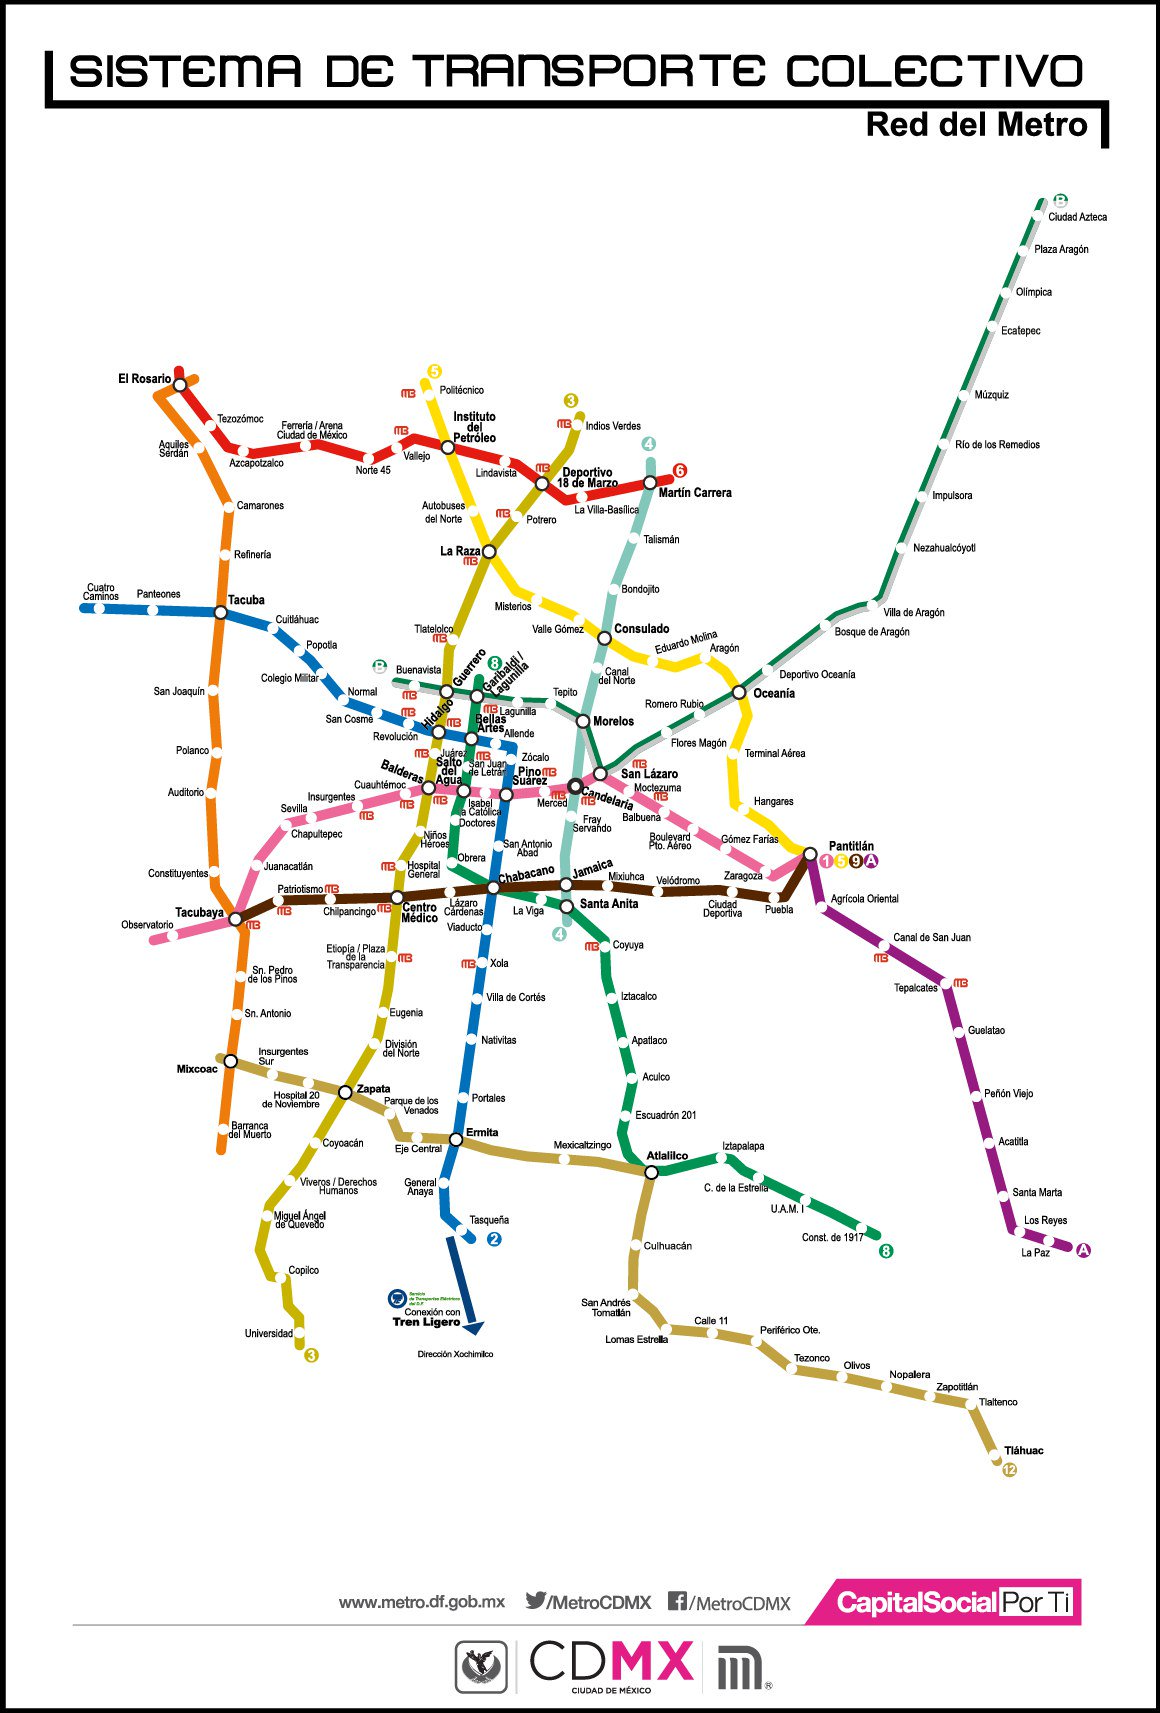
\includegraphics[width=0.6\textwidth,height=3.64583in]{Imagenes/Red_metro_cdmx.png}
\caption{Metro de la CDMX}
\end{figure}

Como usuarios del metro, sabemos que actualmente existe un problema de
saturación, pues sin lugar a dudas tal vez sigue siendo el sistema de
transporte más barato para la pobación en general ya que con 5 pesos es
posible cruzar la ciudad de un extremo a otro. Si bien, el presente
trabajo no pretende dar una solución a dicho problema, si tiene por
objetivo hacer tres tipos de recomendaciones para cualquier usuqrio:

\begin{enumerate}
\def\labelenumi{\arabic{enumi}.}
\tightlist
\item
  La primera recomendación se base en sugerir la ruta más corta en
  distancia en metros
\item
  La segunda recomendación se basa en sugerir al usuario la ruta con
  menos afluencia de personas. Esto con la idea de que el usuario viaje
  un tanto más cómodo considerando que hay menos cantidad de personas en
  el viaje sugerido.
\item
  La última recomendación se base en una combinación de las dos
  anteriores y consiste en ponderar la distancia por el nivel de
  afluencia de personas con el objetivo de sacar una ruta más ``óptima''
  pensando en los dos factores.
\end{enumerate}

Si bien, esta solución no representa necesariamente una solución
universal al los problemas que representa viajar en metro, si es una
gran iniciativa en el afán de querer mejorar la movilidad de los
usuarios.

\hypertarget{soluciuxf3n-teuxf3rica-del-problema}{%
\subsection{Solución teórica del
problema}\label{soluciuxf3n-teuxf3rica-del-problema}}

Tal y como se describe en la introducción de este documento, la idea de
poder resolver este problema consiste en encontrar la ruta más corta de
una estación de metro a otra. En ese orden de ideas podemos pensar a la
red de metro como una red en donde cada estacion respresenta un noda y
la conexión entre cada una de ellas representa un vertice.

El peso de cada uno de los vertices puede estar representado ya sea por
la distancia en metros que separa una estación de la otra o bien, por la
afluencia de personas que puede haber de una estación a otra. Si
pensamos cada estación como los renglones y columnas de una matriz
cuadrada, es fácil ver que tratandose de las distancias la matriz
resultante será simétrica, por lo que que la ruta más corta de la
estación ``A'' a ``B'' será la misma que ir de ``B'' a ``A''.

Contrario a lo que sucede con las distancias, cuando hablamos de la
afluencia de personas la matriz no resulta ser simétrica: esto porque la
afluencia de una estación no es la misma que la de la estación vecina, y
no será lo mismo ir de ``A'' a ``B'' que de ``B'' a ``A''. Un ejemplo
más concreto sería que la afluencia promedio de personas de la estación
``A'' es 10,000 personas en un día mientras que en el caso de B sólo es
de 1000 personas, si yo, como usuario del metro viajo de ``A'' a ``B''
me encontraré más personas al momento de abordar y será menos probable
que alcance un lugar para sentarme o siquiera que pueda subirme al tren,
mientras que si viajo de ``B'' a ``A'' es mucho más factible que suceda
lo contrario, es decir, que alcance algún lugar se vuelve más probable y
más aún, que realmente pueda abordar el tren.

En la literatura existen varios algoritimos que pueden ayudarnos a
resolver este tipo de problemas de encontrar la ruta más corta, tal vez
el uno de los más conocidos sea el método simplex, sin embargo en una
red de nodos tan grande como lo es el metro, puede resultar ser poco
factible, pues la función de optimización a plantear junto con todas las
restricciones puede resultar ser poco manejable.

Existe otro algoritmo del cual se puede encontrar mucha literatura,
publicado en 1959 lleva el nombre de su autor: el algoritmo de Dijkstra.
Este algoritmo fue diseñado para encontrar la ruta más corta en una red
extensa de nodos y a diferencia del método simplex no requiere definir
una función de optimización ni mucho menos.

\hypertarget{explicaciuxf3n-del-algoritmo}{%
\subsubsection{Explicación del
algoritmo}\label{explicaciuxf3n-del-algoritmo}}

La siguiente explicación se basa en
{[}\protect\hyperlink{ref-dijkstra2022note}{1}{]} y
{[}\protect\hyperlink{ref-noauthor_dijkstras_2020}{2}{]}. Básicamente el
algoritmo de Dijkstra comienza en el nodo que el usuario elija (nodo
origen) y analiza el grafo para encontrar la ruta más corta entre dicho
nodo y un nodo destino que también será elejido por el usuario. En
términos generales el funcionamiento es el siguiente
{[}\protect\hyperlink{ref-noauthor_dijkstras_2020}{2}{]}:

\begin{itemize}
\tightlist
\item
  Se comienza en el nodo fuente y se va analizando cada distancia al
  nodo adyacente.
\item
  Se almacena la distancia más corta encontrada hasta el momento
\item
  Se continua con el siguiente nodo más adjacente, se evalúa la
  distancia y se actualizan las distancias mínimas en caso de econtrarse
  una distancia más corta.
\item
  Se repite hasta visitar el nodo más lejano.
\end{itemize}

El algoritmo únicamente puede trabajar con valores positivos en los
pesos, esto porque durante el desarrollo del algoritmo dichos pesos se
irán sumando, si hubiera un caso negativo entronces dicho algoritmo no
funcionaría correctamente pues decir que se ha encontrado la ruta más
corta sería engañoso e incluso podrías caracer de
interpretabilidad.\footnote{Aunque podemos solucionar esto al hacer una
  transformación a los datos como obtener el valor absoluto de los pesos
  dependiendo el contexto}

A contunuación se muestra un ejemplo de como funciona el algoritmo.
Considere el siguiente grafo:

\begin{figure}

{\centering \includegraphics[width=0.5\linewidth,height=0.5\textheight]{Metro_CDMX_files/figure-latex/unnamed-chunk-2-1} 

}

\caption{Ejemplo de red con 6 nodos}\label{fig:unnamed-chunk-2}
\end{figure}

La figura 2 representa una conexión entre 6 nodos, la distancia de cada
uno de ellos esta dado por el número que se puede observa entre sus
vertices, la distancia de ir del nodo 0 al nodo 1 es 2 mientras que ir
del nodo 0 al nodo 2 la distancia es de 6. Dijksta generará la distancia
más corta del nodo 0 a cualquier otro nodo dentro de la red.

Inicializamos el algoritmo, la siguiente tabla muestra las distancias
iniciales para cada nodo:

\begin{longtable}[]{@{}cc@{}}
\toprule()
Nodo & Distancia \\
\midrule()
\endhead
0 & 0 \\
1 & \(\infty\) \\
2 & \(\infty\) \\
3 & \(\infty\) \\
4 & \(\infty\) \\
5 & \(\infty\) \\
6 & \(\infty\) \\
\bottomrule()
\end{longtable}

Note que la distancia inicial en el nodo 0 consigo mismo será 0,
mientras que para el resto las distancias iniciales, dado que estas no
se conocen se inicializan con el simbolo \(\infty\). Por otro lado
definimos la lista de los nodos no visitados: \(\{0,1,2,3,4,5,6 \}\).
Dado que el nodo origen es el nodo 0, lo marcamos como visitado, para
ello usarmos el signo ``-'' dentro de nuestra lista para dentar que
hemos visitado dicho nodo: \(\{-0,1,2,3,4,5,6 \}\).

Ahora, revisamos la distancia que existe entre el nodo 0 y sus nodos
adyacentes, que en este caso son 1 y 2. Una ves que hemos revisado las
distancias, actualizamos nuestra tabla tal que:

\begin{longtable}[]{@{}cc@{}}
\toprule()
Nodo & Distancia \\
\midrule()
\endhead
0 & 0 \\
1 & 2 \\
2 & 6 \\
3 & \(\infty\) \\
4 & \(\infty\) \\
5 & \(\infty\) \\
6 & \(\infty\) \\
\bottomrule()
\end{longtable}

Y posterior a ello, seleccionamos el nodo cuya distancia es menor al
nodo origen, una vez que lo hemos seleccionado marcamos ese nodo como
visitado. Adicional, agregmos un elemento más a la lista, que será la
ruta, en este caso esta irá del nodo 0 al 1 tal que:
\(\{0 \rightarrow 1 \}\) y \(\{-0,-1,2,3,4,5,6 \}\)

Ahora necesitamos analizar los nuevos nodos adyacentes para encontrar el
camino más corto para llegar a ellos. Solo analizaremos los nodos que
son adyacentes a los nodos que ya forman parte del camino más corto. El
nodo 3 y el nodo 2 son adyacentes a los nodos que ya están en la ruta
porque están conectados directamente al nodo 1 y al nodo 0,
respectivamente. Estos son los nodos que analizaremos en el siguiente
paso{[}\protect\hyperlink{ref-noauthor_dijkstras_2020}{2}{]}.

Como ya tenemos la distancia desde el nodo de origen hasta el nodo 2
anotada en nuestra lista, no necesitamos actualizar la distancia esta
vez. Solo necesitamos actualizar la distancia desde el nodo de origen
hasta el nuevo nodo adyacente (nodo 3). Por lo que la tabla resultante
será {[}\protect\hyperlink{ref-noauthor_dijkstras_2020}{2}{]}:

\begin{longtable}[]{@{}cc@{}}
\toprule()
Nodo & Distancia \\
\midrule()
\endhead
0 & 0 \\
1 & 2 \\
2 & 6 \\
3 & 7 \\
4 & \(\infty\) \\
5 & \(\infty\) \\
6 & \(\infty\) \\
\bottomrule()
\end{longtable}

Note que en este caso, la distancia actualizada será 7 pues es el
resultado de la suma de 2 y 5 que es la distancia que nos toma llegar
del nodo 0 al nodo 3. Ahora, de los nodos aún no visitados y basados en
la tabla anterior debemos elegir el que represente la distancia más
corta desde el nodo origen, en este caso la distancia más corta será 6 y
marcamos este como visitado tal que \(\{-0,-1,-2,3,4,5,6 \}\). Ahora
tenemos dos rutas que en este caso son:
\(\{0 \rightarrow 1 \} y \{0 \rightarrow 2\}\), luego entonces debemos
elegir la ruta más corta para llegar al nodo 3.

En nuestra tabla anterior, note que el nodo 3 ya tiene una distancia
derivado de los pasos anteriores, pero ahora tenemos una alternativa que
será considerar la distancia entre el nodo 2 y 3. Por la figura 2, la
suma de estas distancias es de 14, mientras que la distancia ya
registrada anteriormete es de 7 como se observa en la tabal, de forma
que conservamos la ruta que originalmente habìamos tomado y agregamos el
nuevo nodo tal que: \(\{0 \rightarrow 1 \rightarrow 3\}\). Hemos llegado
al nodo 3, así que ahora podemos marcarlo como visitado:
\(\{-0,-1,-2,-3,4,5,6 \}\)

Hasta debemos de revisar las distancias que se derivan de ir a los nodos
no visitados, en este caso para ir al nodo 4 la ruta definida sería
\(\{0 \rightarrow 1 \rightarrow 3 \rightarrow 4\}\) cuya distancia es
17, mientras que para ir al nodo 5 la ruta es
\(\{0 \rightarrow 1 \rightarrow 3 \rightarrow 5\}\) y cuya distancia es
22. Actualizamos de nueva cuenta nuestra tabla de distancias:

\begin{longtable}[]{@{}cc@{}}
\toprule()
Nodo & Distancia \\
\midrule()
\endhead
0 & 0 \\
1 & 2 \\
2 & 6 \\
3 & 7 \\
4 & 17 \\
5 & 22 \\
6 & \(\infty\) \\
\bottomrule()
\end{longtable}

Ahora, debemos marcar como visitado aquel nodo que nos haya dado la
distancia más corta, que en este caso es el nodo 4:
\(\{-0,-1,-2,-3,-4,5,6 \}\) y la ruta actualizada será
\(\{0 \rightarrow 1 \rightarrow 3 \rightarrow 4\}\). Una vez más
repetimos los mismos pasos para el nodo 5 y 6.

Para el nodo 5, la primera opción es seguir la ruta
\(\{0 \rightarrow 1 \rightarrow 3 \rightarrow 5\}\) que tiene una
distancia de 22. La segunda opción será
\(\{0 \rightarrow 1 \rightarrow 3 \rightarrow 4 \rightarrow 5\}\) el
cual la distancia será 23 desde el nodo origen, claramente la primera
ruta es la más corta.

Para el nodo 6 la ruta disponible es
\(\{0 \rightarrow 1 \rightarrow 3 \rightarrow 4 \rightarrow 6\}\) con
una distancia de 19. Ahora marcamos como visitado el nodo con la ruta
más corta, que en este caso será el 6: \(\{-0,-1,-2,-3,-4,5,-6 \}\).
Actualizamos la tabla de distancias:

\begin{longtable}[]{@{}cc@{}}
\toprule()
Nodo & Distancia \\
\midrule()
\endhead
0 & 0 \\
1 & 2 \\
2 & 6 \\
3 & 7 \\
4 & 17 \\
5 & 22 \\
6 & 19 \\
\bottomrule()
\end{longtable}

Finalmente, el único nodo no visitado es el nodo 5, veamos como podemos
incluirlo en la ruta. Existen 3 rutas posibles para llegar del nodo
origen al nodo 5 que son:

\begin{enumerate}
\def\labelenumi{\arabic{enumi}.}
\tightlist
\item
  \(\{0 \rightarrow 1 \rightarrow 3 \rightarrow 5\}\) con distancia de
  22
\item
  \(\{0 \rightarrow 1 \rightarrow 3 \rightarrow 4 \rightarrow 5\}\) con
  distancia de 23
\item
  \(\{0 \rightarrow 1 \rightarrow 3 \rightarrow 4 \rightarrow 6 \rightarrow 5\}\)
  con distancia de 25
\end{enumerate}

Así que la ruta seleccionada para ir del nodo 0 al nodo 5 será la
primera, marcamos este nodo cómo visitado y agregamos esta nueva ruta:
\(\{-0,-1,-2,-3,-4,-5,-6 \}\),
\(\{0 \rightarrow 1 \rightarrow 3 \rightarrow 5\}\). Con ello hemos
encontrado la ruta más corta desde el nodo origen a cualquier otro nodo
dentro de la red. Este mismo principio es el que usaremos para aplicarlo
a nuestro porblema, más detalle de ello se puede ver en la sección de
implementación del algoritmo.

\hypertarget{datos}{%
\subsection{Datos}\label{datos}}

\hypertarget{generaciuxf3n-matriz-de-adyacencias}{%
\subsubsection{Generación Matriz de
Adyacencias}\label{generaciuxf3n-matriz-de-adyacencias}}

Para el ejercicio, se descargó la base de datos de la siguiente liga
\href{https://metro.cdmx.gob.mx/longitud-de-estacion}{liga}, la cual
contiene la relación de las distancias en metros entre las estaciones
del metro de la CDMX, detallando la línea a la que pertenecen y
mostradas de forma ordenada como se muestra a continuación:

\begin{Shaded}
\begin{Highlighting}[]
\NormalTok{distancias }\OtherTok{\textless{}{-}}\FunctionTok{read\_excel}\NormalTok{(}\StringTok{\textquotesingle{}C:/Users/palin/OneDrive/Documentos/MaestriaEnCienciaDeDatos/Semestre3/MétodosNuméricos/FinalAline/Data1/distancia\_metro.xlsx\textquotesingle{}}\NormalTok{)}
\NormalTok{distancias }\SpecialCharTok{\%\textgreater{}\%} \FunctionTok{head}\NormalTok{(}\DecValTok{10}\NormalTok{)}
\end{Highlighting}
\end{Shaded}

\begin{verbatim}
## # A tibble: 10 x 5
##    Linea Estacion1            Estacion2            Long_estacion Long_interest~1
##    <chr> <chr>                <chr>                        <dbl>           <dbl>
##  1 1     Pantitlan            Zaragoza                       150            1320
##  2 1     Zaragoza             GomezFarias                    150             762
##  3 1     GomezFarias          BoulevardPuertoAereo           150             611
##  4 1     BoulevardPuertoAereo Balbuena                       150             595
##  5 1     Balbuena             Moctezuma                      150             703
##  6 1     Moctezuma            SanLazaro                      150             478
##  7 1     SanLazaro            Candelaria                     150             866
##  8 1     Candelaria           Merced                         150             698
##  9 1     Merced               PinoSuarez                     150             745
## 10 1     PinoSuarez           IsabellaCatolica               150             382
## # ... with abbreviated variable name 1: Long_interestacion
\end{verbatim}

Para poder generar la matriz de adyacencias, se consideraron como los
nodos todas las estaciones (164), y los pesos para cada una el campo
``Long\_interestacion'', que contiene la distancia entre cada estación,
esta matriz será simétrica, pues en términos de esta medida es lo mismo
ir de Pantitlán a Zaragoza que viceversa. Dado que la matriz es muy
grande para ser visualizada, puede consultarse en la carpeta Matrices en
el repositorio de GitHub.

En realidad la construcción de esta matriz fue bastante directa y con
ella buscamos encontrar la ruta más corta.

\hypertarget{generaciuxf3n-matriz-de-afluencias}{%
\subsubsection{Generación Matriz de
Afluencias}\label{generaciuxf3n-matriz-de-afluencias}}

Como complemento al modelo original y queriendo responder preguntas
como: ¿Que ruta es más cómoda en términos de afluencia de personas?, es
decir que pasa si como usuario del metro me interesa más que la ruta más
corta la ruta más cómoda en términos del número de personas que la
transitan.

Bajo este enfoque nos interesa agregar la siguiente base tomada de
\url{https://datos.cdmx.gob.mx/dataset/afluencia-diaria-del-metro-cdmx}
, Esta base muestra la afluencia diaria del Metro CDMX. Los datos se
encuentran actualizados al 1 de diciembre de 2022 y su profundidad
histórica abarca desde enero 2010 al 31 de octubre 2022.

La base de afluencia desglosada se refiere a la afluencia en el
Organismo Público de Transporte STC Metro, separada por medio de acceso,
los cuales son: Tarjeta Única de Movilidad Integrada, boleto y
gratuidad, esta última se refiere al acceso gratuito para las personas
adultos mayores, personas con discapacidad y/o niños menores de 5 años,
de acuerdo a los requisitos establecidos por el Organismo.

\begin{Shaded}
\begin{Highlighting}[]
\NormalTok{afluencia }\OtherTok{\textless{}{-}}\FunctionTok{read\_csv}\NormalTok{(}\StringTok{\textquotesingle{}C:/Users/palin/OneDrive/Documentos/MaestriaEnCienciaDeDatos/Semestre3/MétodosNuméricos/FinalAline/Data1/afluenciastc\_simple\_01\_12\_2022.csv\textquotesingle{}}\NormalTok{)}
\NormalTok{afluencia }\SpecialCharTok{\%\textgreater{}\%} \FunctionTok{head}\NormalTok{(}\DecValTok{10}\NormalTok{)}
\end{Highlighting}
\end{Shaded}

\begin{verbatim}
## # A tibble: 10 x 6
##    fecha       anio mes   linea   estacion            afluencia
##    <chr>      <dbl> <chr> <chr>   <chr>                   <dbl>
##  1 01/01/2010  2010 Enero Linea 1 Zaragoza                20227
##  2 01/01/2010  2010 Enero Linea 1 Isabel la Católica       6487
##  3 01/01/2010  2010 Enero Linea 1 Moctezuma               10304
##  4 01/01/2010  2010 Enero Linea 1 Pino Suárez              8679
##  5 01/01/2010  2010 Enero Linea 1 Gómez Farías            19499
##  6 01/01/2010  2010 Enero Linea 6 Deptvo. 18 de Marzo       621
##  7 01/01/2010  2010 Enero Linea 6 La Villa-Basilica       24792
##  8 01/01/2010  2010 Enero Linea 9 Pantitlán               27000
##  9 01/01/2010  2010 Enero Linea 8 Aculco                   3652
## 10 01/01/2010  2010 Enero Linea 9 Velódromo                3239
\end{verbatim}

Por ejemplo podemos ver el top 5 de las estaciones con mayor afluencia
para el día más reciente en la base `2022-10-31', sin considerar la
linea:

\begin{Shaded}
\begin{Highlighting}[]
\NormalTok{afluencia}\SpecialCharTok{$}\NormalTok{fecha }\OtherTok{\textless{}{-}} \FunctionTok{as.Date}\NormalTok{(afluencia}\SpecialCharTok{$}\NormalTok{fecha,}\AttributeTok{format =} \StringTok{"\%d/\%m/\%Y"}\NormalTok{)}
\NormalTok{afluencia }\SpecialCharTok{\%\textgreater{}\%} \FunctionTok{filter}\NormalTok{(fecha}\SpecialCharTok{==}\StringTok{\textquotesingle{}2022{-}10{-}31\textquotesingle{}}\NormalTok{) }\SpecialCharTok{\%\textgreater{}\%}  \FunctionTok{group\_by}\NormalTok{(estacion) }\SpecialCharTok{\%\textgreater{}\%} \FunctionTok{summarise}\NormalTok{(}\AttributeTok{Afluencias\_suma =} \FunctionTok{sum}\NormalTok{(afluencia)) }\SpecialCharTok{\%\textgreater{}\%} \FunctionTok{arrange}\NormalTok{(}\FunctionTok{desc}\NormalTok{(Afluencias\_suma)) }\SpecialCharTok{\%\textgreater{}\%} \FunctionTok{head}\NormalTok{(}\DecValTok{5}\NormalTok{)}
\end{Highlighting}
\end{Shaded}

\begin{verbatim}
## # A tibble: 5 x 2
##   estacion             Afluencias_suma
##   <chr>                          <dbl>
## 1 Pantitlán                     159357
## 2 Indios Verdes                 102621
## 3 Constitución de 1917           87075
## 4 Tacubaya                       81492
## 5 Tasqueña                       73599
\end{verbatim}

Ahora observemos el primer lugar de acuerdo a la linea del metro, por
ejemplo Pantitlán que tiene varios cruces de lineas

\begin{Shaded}
\begin{Highlighting}[]
\NormalTok{afluencia }\SpecialCharTok{\%\textgreater{}\%} \FunctionTok{filter}\NormalTok{((fecha}\SpecialCharTok{==}\StringTok{\textquotesingle{}2022{-}10{-}31\textquotesingle{}}\NormalTok{)}\SpecialCharTok{\&}\NormalTok{(}\FunctionTok{str\_detect}\NormalTok{(estacion,}\StringTok{"Pantitl"}\NormalTok{)))}
\end{Highlighting}
\end{Shaded}

\begin{verbatim}
## # A tibble: 4 x 6
##   fecha       anio mes     linea   estacion  afluencia
##   <date>     <dbl> <chr>   <chr>   <chr>         <dbl>
## 1 2022-10-31  2022 Octubre Linea 1 Pantitlán         0
## 2 2022-10-31  2022 Octubre Linea 5 Pantitlán     51160
## 3 2022-10-31  2022 Octubre Linea 9 Pantitlán     61233
## 4 2022-10-31  2022 Octubre Linea A Pantitlán     46964
\end{verbatim}

Observemos como se comporta la afluencia de una de las estaciones más
caóticas de la CDMX

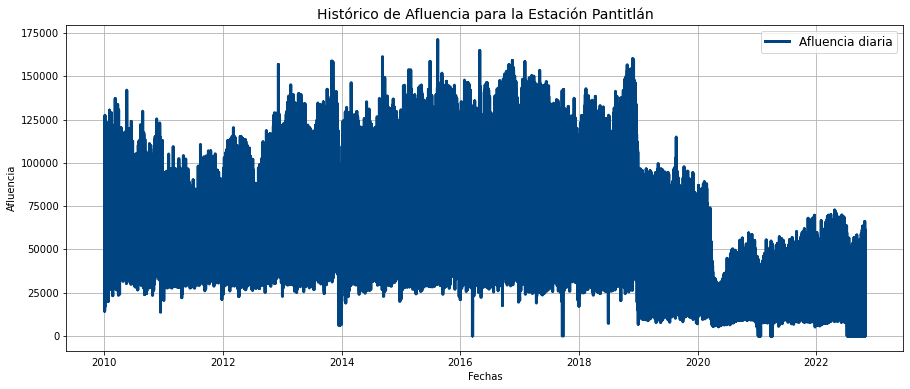
\includegraphics[width=0.6\textwidth,height=3.64583in]{Imagenes/Pantitlan.png}
Indios Verdes es otra de las estaciones con mayor afluencia
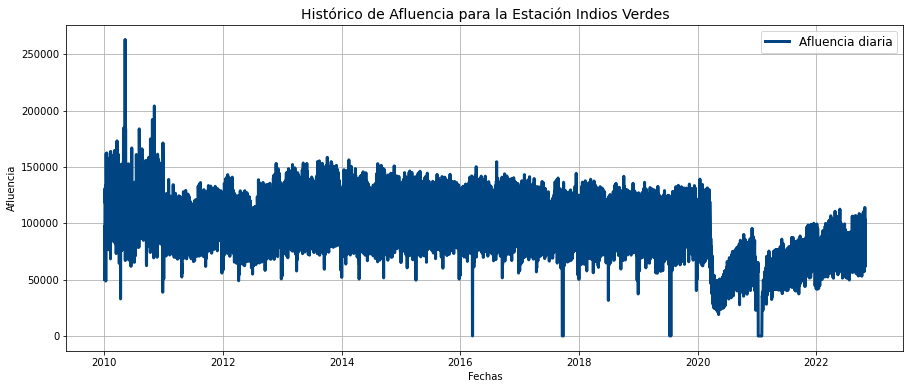
\includegraphics[width=0.6\textwidth,height=3.64583in]{Imagenes/IndiosVerdes.png}
Observemos que Pantitlán por ejemplo es una de las estaciones que
históricamente ha tenido mayor afluencia de personas, también podemos
notar que antes de la pandemia, la concentración de personas era mucho
mayor, que post-Covid. Esto nos lleva a preguntarnos como integrar esta
información en nuestros datos dado que históricamente cada estación
tiene una afluencia distinta. Lo más sencillo es cortar nuestra
información a partir de mediados 2021 donde la movilidad empieza a
estabilizarse debido a que la pandemia comienza su desaceleración, de
esta manera podemos tomarnos como valor fijo entre nodos la mediana de
los datos, para este rango de fechas, siendo este un mejor estimador que
la media.

Sabemos además que las estaciones con mayores transbordos como lo es
pantitlán van a presentar mayor afluencia y esta dependerá de la línea
en la que viajen, para fines prácticos de este ejercicio, se asumirá
pantitlán como un solo nodo sin importar la línea en la que te
encuentras.

Supondremos además que la afluencia tiene dirección, es decir si vas en
la línea 1 por ejemplo de Pantitlán a Zaragoza, sabemos que la mediana
de afluencia en Pantitlán es n, así que la afluencia de Pantitlán a
Zaragoza será n, y si la afluencia de Zaragoza es m y su dirección es
pantitlán, entonces la afluencia de esa dirección será m.

Este quizá sea uno de los supuestos más grandes al integrar esta matriz
al modelo, pues estamos haciendo el supuesto de que la cantidad de
personas que se reportan entran a una estación permanecen en la
siguiente, cuando sabemos que en la realidad esto no necesariamente es
cierto, pues si n personas suben en Pantitlán, tienen muchas opciones
para moverse, ya que esa estación tiene 4 transbordos, es decir, 4
líneas contiguas, su siguiente opción puede ser Zaragoza, Agrícola
Oriental, Puebla o Hangares, sin embargo, al no contar con este nivel de
detalle en bases públicas, abordaremos este problema de la siguiente
forma:

\begin{enumerate}
\def\labelenumi{\arabic{enumi}.}
\item
  Una opción de matriz será bajo el supuesto de que las personas que
  entran a x estación permanecen en la siguiente.
\item
  Dado que cada estación tiene una afluencia diferente, se desarrollará
  una segunda matriz que contemple tanto las distancias previamente
  desarrolladas, como la proporción de afluencia de cada estación. Dicha
  proporción será considera de acuerdo a líneas completas, es decir, si
  la línea 1 tiene una afluencia total z, entonces cada una de sus
  estaciones tendrá un peso distinto de acuerdo a su afluencia
  individual, n/z.
\end{enumerate}

Adicional a lo anterior no estamos considerando horarios, la afluencia
es el número de personas totales al día, sin considerar que en horarios
6-9 am o 6-9 pm, son horarios de mucho mayor cocentración de personas
por las horas laborales entre semana y varian bastante los fines de
semana.

Antes de determinar la mediana general por estación, recordemos que el
rango de fechas que estamos considerando es a partir de mediados de
2021, sin embargo, para una estación en particular: línea 12, sufrió un
incidente en mayo 2021, dejándola fuera de servicio a partir de ese
periodo, podemos observar en el siguiente gráfico como se ve su
comportamiento de afluencia histórica. Con fines de no sacarla de
nuestro análisis, pues contamos con su matriz de distancias, decidimos
tomar un periodo distinto únicamente para esta línea, que contemple el
mismo número de periodos (16) y que no se intersecte con la pandemia:
mediados de junio 2018 a 2020.

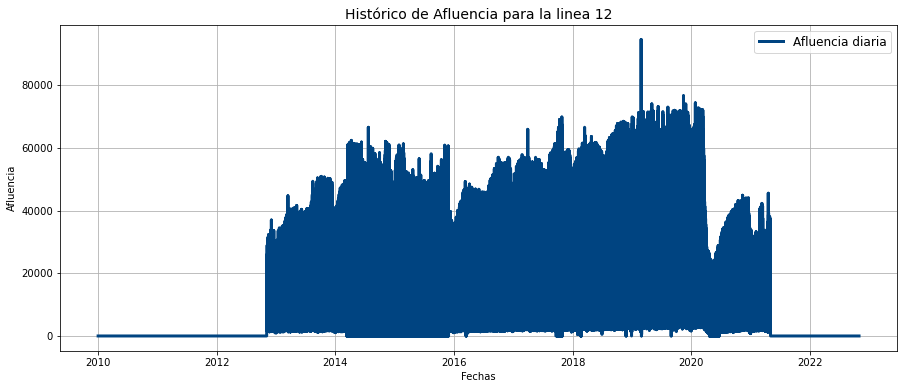
\includegraphics[width=0.6\textwidth,height=3.64583in]{Imagenes/Linea12.png}
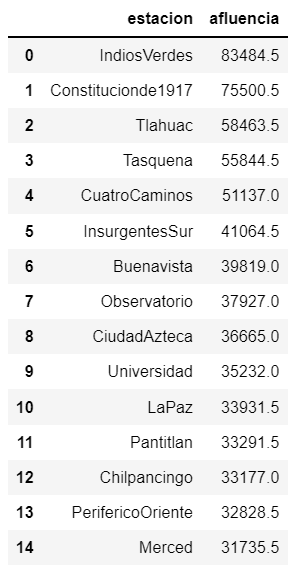
\includegraphics[width=0.4\textwidth,height=5.20833in]{Imagenes/Tabla_medianas.png}
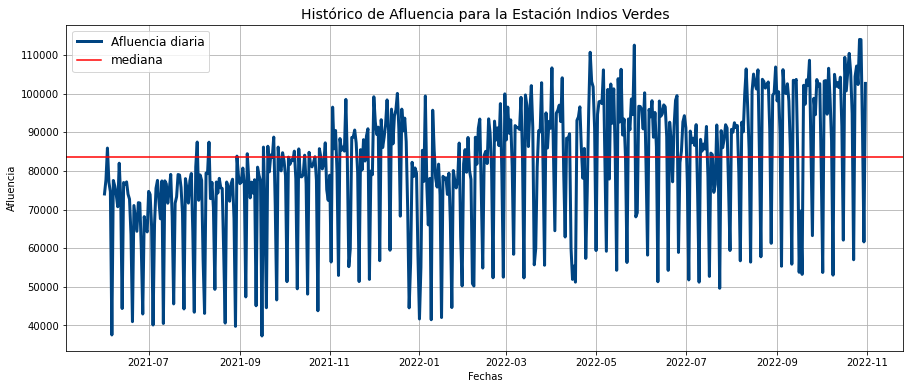
\includegraphics[width=0.4\textwidth,height=5.20833in]{Imagenes/IndiosVerdesMediana.png}

\begin{figure}
\centering
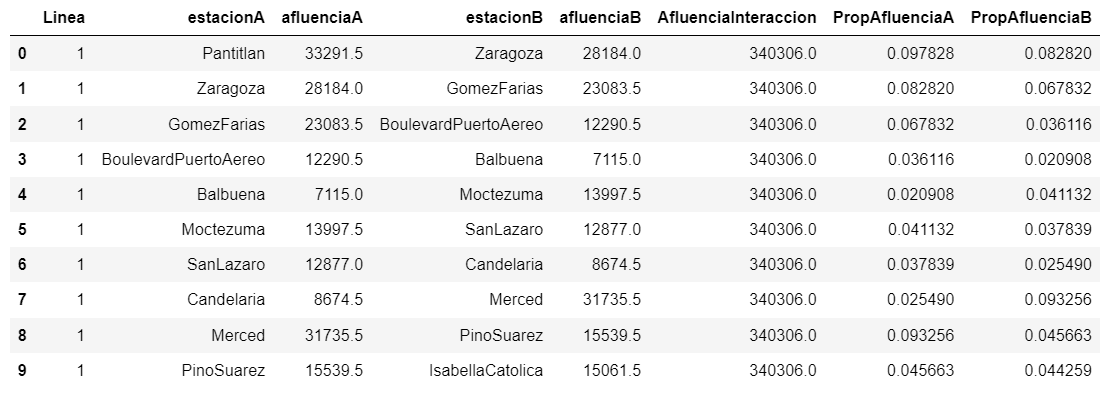
\includegraphics{Imagenes/AfluenciasTable.png}
\caption{Tabla de Afluencias Finales}
\end{figure}

\hypertarget{implementaciuxf3n-del-algoritmo}{%
\subsection{Implementación del
algoritmo}\label{implementaciuxf3n-del-algoritmo}}

Para poder plantear una solución al problema, se hizo uso de los
algoritmos ya existentes definidos por la comunidad científca. En esta
caso, nos basamos en la función \emph{dijkstra\_path} cuya documentación
podemos encontrar en
{[}\protect\hyperlink{ref-noauthor_dijkstra_path_nodate}{3}{]}. Dicha
función trabaja con redes definidas en python y aplica el mismo
principio que se explicó en la sección anterior.

Se plantea la solución a 3 situaciones que bajo un mismo contexto
proponen soluciones diferentes y son:

\begin{enumerate}
\def\labelenumi{\arabic{enumi}.}
\tightlist
\item
  Encontrar la ruta más corta con base en la distancia.
\item
  Encontrar la ruta más ``cómoda'' con base en aquella con menor
  afluencia de personas.
\item
  Proponer una ruta óptima considerando la combinación de los dos puntos
  anteriores.
\end{enumerate}

Para el caso del punto 3, la idea de ruta óptima es un criterio propio
como resultado de la combinación de la distancia y la afluencia de
personas por cada una de las estaciones. Los datos de entrada, ya sea
considerando la distancia entre estaciones o bien el número de personas
se convierten a una matriz de la siguente forma:

\begin{figure}
\centering
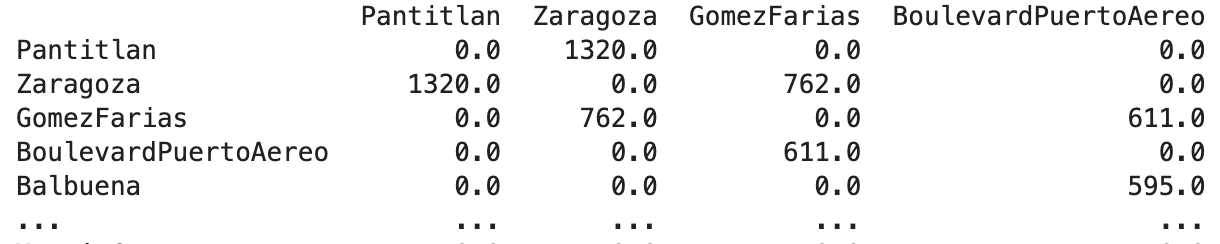
\includegraphics[width=0.6\textwidth,height=3.64583in]{Imagenes/matrix_imagen.png}
\caption{Matriz de adyacencias}
\end{figure}

Si existe una conexión entre una estación y otra se muestra un valor
positivo que indica, según sea el caso, la distancia, la afluencia de
personas o una combinación de ambas. Estás entradas deben ser positivas
o bien cero pues es un requisito que debe cumplirse para que el
algoritmo funcione correctamente (ver Explicación del algoritmo).

Posterior a ello, se arma un arreglo que será el input para armar los
nodos y los vertices de una grafo. Se toma la matriz de adyacencias y se
genera una salida como la que sigue:

\begin{figure}
\centering
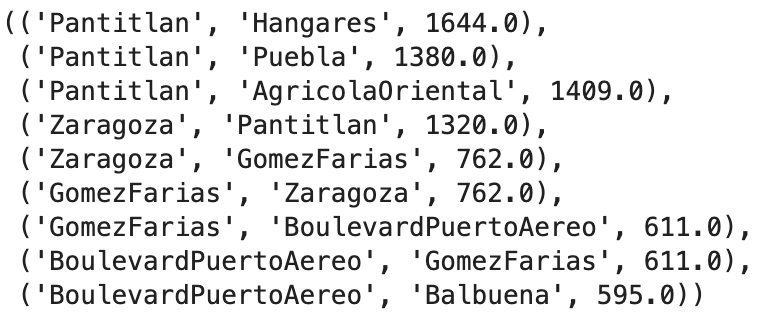
\includegraphics[width=0.6\textwidth,height=3.64583in]{Imagenes/input_nodos_vertices.png}
\caption{Nodos y pesos por cada vertice}
\end{figure}

La figura 2 es sólo una muestra de todos los nodos y pesos definidos,
por ejemplo podemos ver que existe una conección entre el nodo
``Pantitlan'' y el nodo ``Hangares'' cuyo peso (distancia en este caso)
es de 1644 metros.

La salida anterior es la base para generar el grafo que será utilizado
para poder encontrar la ruta más corta en donde, como ya se mencionó
cada estación representa un nodo, existe un vertice dentro de cada uno
de ellos siempre que los pesos entre ambos sea positivo. La siguiente
figura muestra la red de nodos completa para el metro de la CDMX.

\begin{figure}
\centering
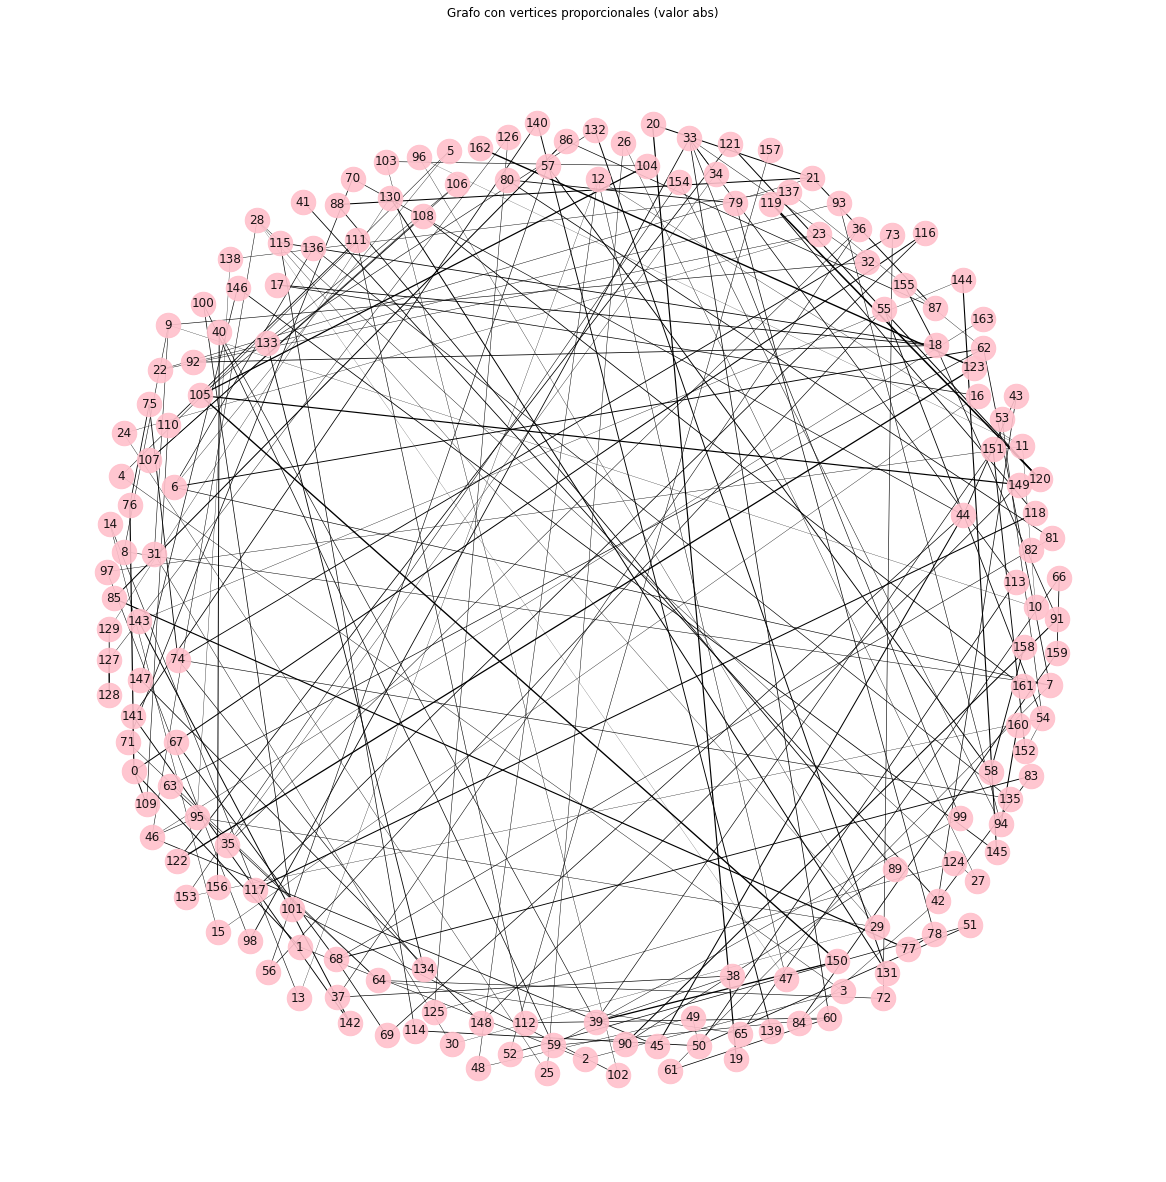
\includegraphics[width=0.6\textwidth,height=3.64583in]{Imagenes/Grafo_v1.png}
\caption{Representación del Metro en un Gráfo}
\end{figure}

Una vez definido red se hace uso de la función meniconada al inicio de
esta sección. La función recibe como parámetro un grafo, el nombre de
una estación del metro que sea el origen y una estación destino tal y
como se muestra a continuación:

\begin{figure}
\centering
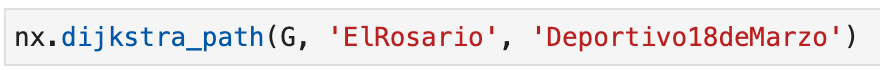
\includegraphics[width=0.6\textwidth,height=\textheight]{Imagenes/dijkstra_function.png}
\caption{Función dikjstra}
\end{figure}

\hypertarget{resultados-y-conclusiones}{%
\subsection{Resultados y conclusiones}\label{resultados-y-conclusiones}}

Los resultados que se derivan de la implementación del modelo se
muestran como en la figura 6, en donde de froma descendente cada entrada
indica la siguiente estación que se deberá tomar para llegar a la
estación de destino ya sea porque se ha tomado la ruta más corta, la
ruta con menor afluencia o la ruta que hemos denonimado la más óptima en
tiempo y confort.

\begin{figure}
\centering
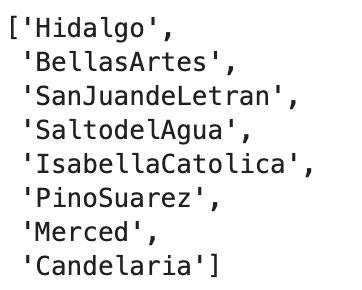
\includegraphics[width=0.3\textwidth,height=1.5625in]{Imagenes/Ejemplo_salida.png}
\caption{Salida del algoritmo: rtua más corta de Hidalgo a Candelaria}
\end{figure}

El ejemplo anterior resulta interesante porque implicaría hacer
transbordes entre líneas que uno como usuario podría pensar que no son
necesarios o que resultan ser más tediosos. Para el ejemplo anterior, la
siguiente imagen muestra dentro del mapa de la red del metro marcada en
rojo, la ruta sugerida para llegar al destino planteado:

\begin{figure}
\centering
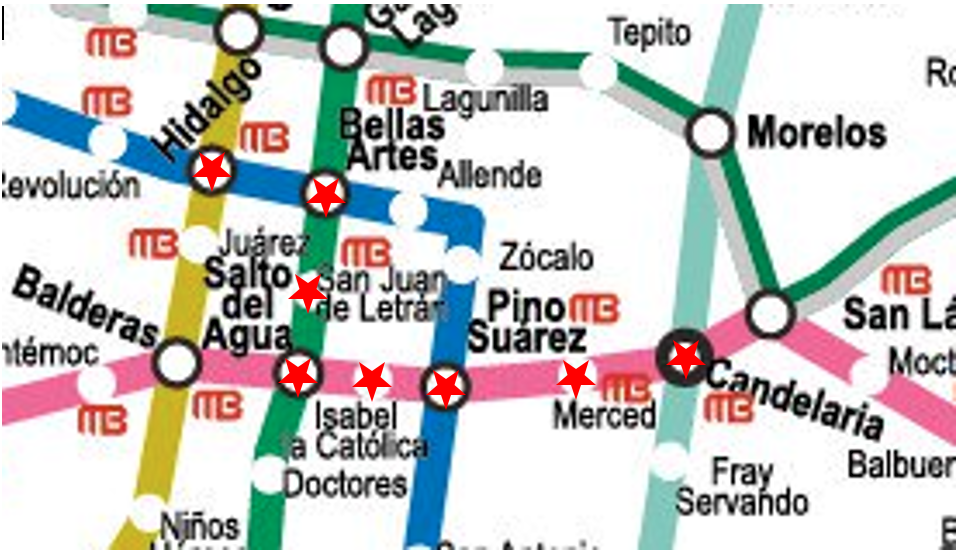
\includegraphics[width=0.6\textwidth,height=3.64583in]{Imagenes/Ruta_sugerida.png}
\caption{Ruta sugerida}
\end{figure}

Note que conseguir ir por la ruta más corta implica hacer un par de
transbordes, el primero de la línea azul a la verde en la esación Bellas
Artes, el segundo sería en Salto del Agua hacia la línea rosa y de ahí
sobre esa misma ruta hasta llegar a Candelaria, sin embargo es probable
que resulte ser más conveniente hacer sólo un transborde pues representa
una situación más cómoda y se hace menos tiempo en llegar al destino que
seguir la ruta más corta.

Escenarios como este plantean agregar otro tipo de datos como lo es el
tiempo promedio de transborde entre estaciones. Como éste caso, puede
haber muchas otras situaciones que sin duda enriquecen la solución al
problema planteado, pero que para fines de este trabajo han quedado
fuera del scope.

\hypertarget{referencias}{%
\subsection*{Referencias}\label{referencias}}
\addcontentsline{toc}{subsection}{Referencias}

\hypertarget{refs}{}
\begin{CSLReferences}{1}{0}
\leavevmode\vadjust pre{\hypertarget{ref-dijkstra2022note}{}}%
1. Dijkstra, E. W. (2022). A note on two problems in connexion with
graphs. In \emph{Edsger wybe dijkstra: His life, work, and legacy} (pp.
287--290).

\leavevmode\vadjust pre{\hypertarget{ref-noauthor_dijkstras_2020}{}}%
2. Dijkstra's {Shortest} {Path} {Algorithm} - {A} {Detailed} and
{Visual} {Introduction}. (2020). In \emph{freeCodeCamp.org}.
\url{https://www.freecodecamp.org/news/dijkstras-shortest-path-algorithm-visual-introduction/}

\leavevmode\vadjust pre{\hypertarget{ref-noauthor_dijkstra_path_nodate}{}}%
3. \emph{Dijkstra\_path --- {NetworkX} 2.8.8 documentation}. (n.d.).
Retrieved December 5, 2022, from
\url{https://networkx.org/documentation/stable/reference/algorithms/generated/networkx.algorithms.shortest_paths.weighted.dijkstra_path.html}

\leavevmode\vadjust pre{\hypertarget{ref-sanchez_mapa_2012}{}}%
4. Sanchez, G. (2012). Mapa del metro del {DF} con {RgoogleMaps}? In
\emph{Mextadísticas}.
\url{https://mextatistics.wordpress.com/2012/05/10/mapa-del-metro-del-df-en-rgooglemaps/}

\end{CSLReferences}

\end{document}
